% Options for packages loaded elsewhere
\PassOptionsToPackage{unicode}{hyperref}
\PassOptionsToPackage{hyphens}{url}
\PassOptionsToPackage{dvipsnames,svgnames,x11names}{xcolor}
%
\documentclass[
]{agujournal2019}

\usepackage{amsmath,amssymb}
\usepackage{iftex}
\ifPDFTeX
  \usepackage[T1]{fontenc}
  \usepackage[utf8]{inputenc}
  \usepackage{textcomp} % provide euro and other symbols
\else % if luatex or xetex
  \usepackage{unicode-math}
  \defaultfontfeatures{Scale=MatchLowercase}
  \defaultfontfeatures[\rmfamily]{Ligatures=TeX,Scale=1}
\fi
\usepackage{lmodern}
\ifPDFTeX\else  
    % xetex/luatex font selection
\fi
% Use upquote if available, for straight quotes in verbatim environments
\IfFileExists{upquote.sty}{\usepackage{upquote}}{}
\IfFileExists{microtype.sty}{% use microtype if available
  \usepackage[]{microtype}
  \UseMicrotypeSet[protrusion]{basicmath} % disable protrusion for tt fonts
}{}
\makeatletter
\@ifundefined{KOMAClassName}{% if non-KOMA class
  \IfFileExists{parskip.sty}{%
    \usepackage{parskip}
  }{% else
    \setlength{\parindent}{0pt}
    \setlength{\parskip}{6pt plus 2pt minus 1pt}}
}{% if KOMA class
  \KOMAoptions{parskip=half}}
\makeatother
\usepackage{xcolor}
\setlength{\emergencystretch}{3em} % prevent overfull lines
\setcounter{secnumdepth}{5}
% Make \paragraph and \subparagraph free-standing
\ifx\paragraph\undefined\else
  \let\oldparagraph\paragraph
  \renewcommand{\paragraph}[1]{\oldparagraph{#1}\mbox{}}
\fi
\ifx\subparagraph\undefined\else
  \let\oldsubparagraph\subparagraph
  \renewcommand{\subparagraph}[1]{\oldsubparagraph{#1}\mbox{}}
\fi


\providecommand{\tightlist}{%
  \setlength{\itemsep}{0pt}\setlength{\parskip}{0pt}}\usepackage{longtable,booktabs,array}
\usepackage{calc} % for calculating minipage widths
% Correct order of tables after \paragraph or \subparagraph
\usepackage{etoolbox}
\makeatletter
\patchcmd\longtable{\par}{\if@noskipsec\mbox{}\fi\par}{}{}
\makeatother
% Allow footnotes in longtable head/foot
\IfFileExists{footnotehyper.sty}{\usepackage{footnotehyper}}{\usepackage{footnote}}
\makesavenoteenv{longtable}
\usepackage{graphicx}
\makeatletter
\def\maxwidth{\ifdim\Gin@nat@width>\linewidth\linewidth\else\Gin@nat@width\fi}
\def\maxheight{\ifdim\Gin@nat@height>\textheight\textheight\else\Gin@nat@height\fi}
\makeatother
% Scale images if necessary, so that they will not overflow the page
% margins by default, and it is still possible to overwrite the defaults
% using explicit options in \includegraphics[width, height, ...]{}
\setkeys{Gin}{width=\maxwidth,height=\maxheight,keepaspectratio}
% Set default figure placement to htbp
\makeatletter
\def\fps@figure{htbp}
\makeatother

\usepackage{url} %this package should fix any errors with URLs in refs.
\usepackage{lineno}
\usepackage[inline]{trackchanges} %for better track changes. finalnew option will compile document with changes incorporated.
\usepackage{soul}
\linenumbers
\makeatletter
\@ifpackageloaded{caption}{}{\usepackage{caption}}
\AtBeginDocument{%
\ifdefined\contentsname
  \renewcommand*\contentsname{Table of contents}
\else
  \newcommand\contentsname{Table of contents}
\fi
\ifdefined\listfigurename
  \renewcommand*\listfigurename{List of Figures}
\else
  \newcommand\listfigurename{List of Figures}
\fi
\ifdefined\listtablename
  \renewcommand*\listtablename{List of Tables}
\else
  \newcommand\listtablename{List of Tables}
\fi
\ifdefined\figurename
  \renewcommand*\figurename{Figure}
\else
  \newcommand\figurename{Figure}
\fi
\ifdefined\tablename
  \renewcommand*\tablename{Table}
\else
  \newcommand\tablename{Table}
\fi
}
\@ifpackageloaded{float}{}{\usepackage{float}}
\floatstyle{ruled}
\@ifundefined{c@chapter}{\newfloat{codelisting}{h}{lop}}{\newfloat{codelisting}{h}{lop}[chapter]}
\floatname{codelisting}{Listing}
\newcommand*\listoflistings{\listof{codelisting}{List of Listings}}
\makeatother
\makeatletter
\makeatother
\makeatletter
\@ifpackageloaded{caption}{}{\usepackage{caption}}
\@ifpackageloaded{subcaption}{}{\usepackage{subcaption}}
\makeatother
\ifLuaTeX
  \usepackage{selnolig}  % disable illegal ligatures
\fi
\usepackage{bookmark}

\IfFileExists{xurl.sty}{\usepackage{xurl}}{} % add URL line breaks if available
\urlstyle{same} % disable monospaced font for URLs
\hypersetup{
  pdftitle={Unlocking Smart Growth: The Effects of Proposed Transit-Oriented Development Laws on the Puget Sound Region},
  pdfauthor={Tiernan Martin},
  pdfkeywords={Transit-Oriented Development, Puget Sound
Region, Washington State 2024 Legislative Session},
  colorlinks=true,
  linkcolor={blue},
  filecolor={Maroon},
  citecolor={Blue},
  urlcolor={Blue},
  pdfcreator={LaTeX via pandoc}}

\journalname{Futurewise}

\draftfalse

\begin{document}
\title{Unlocking Smart Growth: The Effects of Proposed Transit-Oriented
Development Laws on the Puget Sound Region}

\authors{Tiernan Martin\affil{1}}
\affiliation{1}{Futurewise, }
\correspondingauthor{Tiernan Martin}{tiernan@futurewise.org}


\begin{abstract}
During the 2024 legislative session in Washington State, two bills were
introduced in both the House and the Senate aimed at promoting community
and transit-oriented housing development. These bills, HB 2160 and SB
6024, propose mandating cities to permit developments of a specific
scale within certain distances from high-capacity transit stops. This
study evaluates the extent to which the proposed increases in
development capacity under these bills exceed current allowances. The
findings indicate a substantial enhancement in development potential for
the majority of areas within walking distance of transit stops.
Specifically, for land that is developable and presently zoned for lower
development capacity than what the bills propose, the average increase
in capacity is projected to be +1.35 in terms of floor area ratio (FAR).
\end{abstract}

\section*{Plain Language Summary}
In 2024, the Washington State Legislature considered two new laws aimed
at making it easier to build homes near public transit areas, like light
rail stations and bus rapid transit stops. These laws would require
cities to allow taller, denser buildings in these areas. Our study
looked at how much more development could happen under these new laws
compared to what's currently allowed. We found that, if these laws pass,
there would be a lot more room for building new homes and apartments
near transit stops.



\textsubscript{Source:
\href{https://tiernanmartin.github.io/2024-transit-oriented-development-bill/index.qmd.html}{Article
Notebook}}

\subsection*{Acknowledgments}\label{acknowledgments}
\addcontentsline{toc}{subsection}{Acknowledgments}

The authors received no financial support for the research, authorship,
and/or publication of this article.

Thanks to Yonah Freemark from the Urban Institute for providing zoning
district data. Thanks to Lauren Engel, Carol Naito, and Robin Koskey
from the Puget Sound Regional Council for sharing their agency's own
\href{https://arcg.is/0SSvK10}{analysis} of HB 2160/SB 6024. Thanks to
Noha Mahgoub from the Office of Governor Jay Inslee for providing
feedback and guidance.

\subsection{Introduction}\label{introduction}

\begin{figure}[H]

{\centering 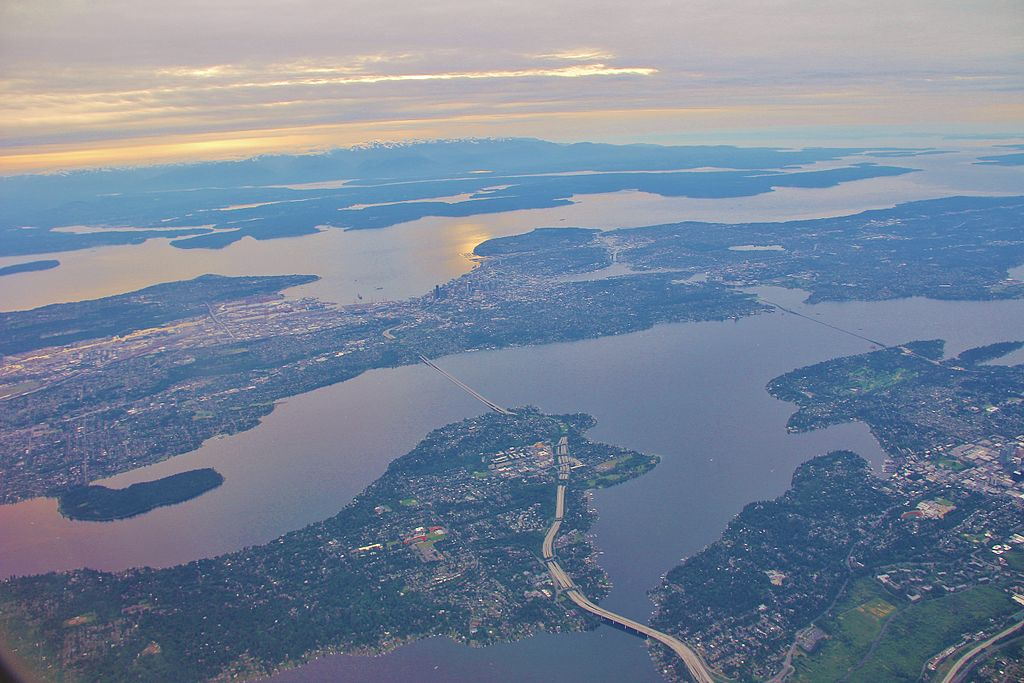
\includegraphics{images/seattle-aerial-wikicommons.jpg}

}

\caption{Central Puget Sound \textbar{} Photo courtesy of
\hyperref[0]{Clemens Vasters from Viersen, Germany}, \hyperref[0]{CC BY
2.0}, via Wikimedia Commons}

\end{figure}%

\textsubscript{Source:
\href{https://tiernanmartin.github.io/2024-transit-oriented-development-bill/index.qmd.html}{Article
Notebook}}

The Puget Sound metropolitan region attracts jobs and residents at some
of the highest rates in North America. Between 2010 and 2022, the
region's population grew by 620,979 people (17\%).\footnote{Population
  statistic calculated by the author based on analysis of data from the
  US 2010 Decennial Census and the US 2022 American Community Survey.}

\subsection{Data \& Methods}\label{sec-data-methods}

\subsection{Results}\label{results}

\subsection{Discussion}\label{discussion}

\subsection{Conclusion}\label{conclusion}

\subsection*{Notes}\label{notes}
\addcontentsline{toc}{subsection}{Notes}

\subsection*{References}\label{references}
\addcontentsline{toc}{subsection}{References}



\end{document}
